\documentclass[10pt]{article}
\usepackage{latexsym}
\usepackage{natbib}
\usepackage{graphicx}
\usepackage{subfigure}
\usepackage{listings}
\usepackage{algorithm}
\usepackage{algpseudocode}
\usepackage{booktabs}
\usepackage{multirow}
\usepackage{siunitx}

\title{Homework 3: Active Learning for Statistical Parsing}
\author{Yu Feng}
\date{4-7-2015}

\begin{document}
\maketitle

\section{Introduction}\label{sec:intro}
The goal of active learning is to get good performance while using as few training
examples as possible. The key idea behind it is to pick training examples in a 
smart way by using different selection functions.

In this report, I explore the performance of four different types of selection
 functions through the WSJ corpus.
 
\section{Four selection functions for active learning}\label{sec:alg}
The key insight of active learning is to pick up the sample with the highest 
uncertainty.  
\subsection{Random Selection $T_{ran}$}
This is just to pick up samples from training set randomly and it's supposed to be
the baseline. But based on the following experimental results, random selection
can also achieve moderate results in some scenarios.

\subsection{Sentence Length $T_{len}$}
A naive method which uses the number of words in a sentence to measure the uncertainty.

\subsection{Normalized probability of the top parse $T_{prob}$}
Using the probability of the selected parse tree to measure the uncertainty and lower 
probability denotes higher uncertainty. To get a fair choice, I normalized the 
probability by taking its $(n-1)$th root.

\subsection{Tree Entropy $T_{tree}$}
Tree entropy~\cite{hwa} uses the probability distribution across all parse trees of a
sentence to measure uncertainty. For more details of the algorithm, please refer to 
the original paper.


\section{Experiments}\label{sec:exp}
In this section I will design different experiments for statical parsing to evaluate the performance of the above four selection functions that are used in active learning. 
All the experiments were ran on the server at Stanford University(\texttt{kuhu2.stanford.edu}). For simplicity, in the following sections we will use $T_{ran}$(Random), $T_{len}$(Length), $T_{prob}$(TopParser) and 
$T_{Tree}$(Tree) to refer the four selection functions in section~\ref{sec:alg}, respectively.


\subsection{Basic experiment}
{\bf \emph{Basic characteristics.}} First I used the first 50 sentences from WSJ 
section 00 as the initial training set and sections 01-03 as the training pool.
For all four section methods, 1500 words are selected from the training pool during 
each iteration and the parser was tested it on WSJ section 20. I executed 20 iterations in total.

 \begin{figure}
\centering
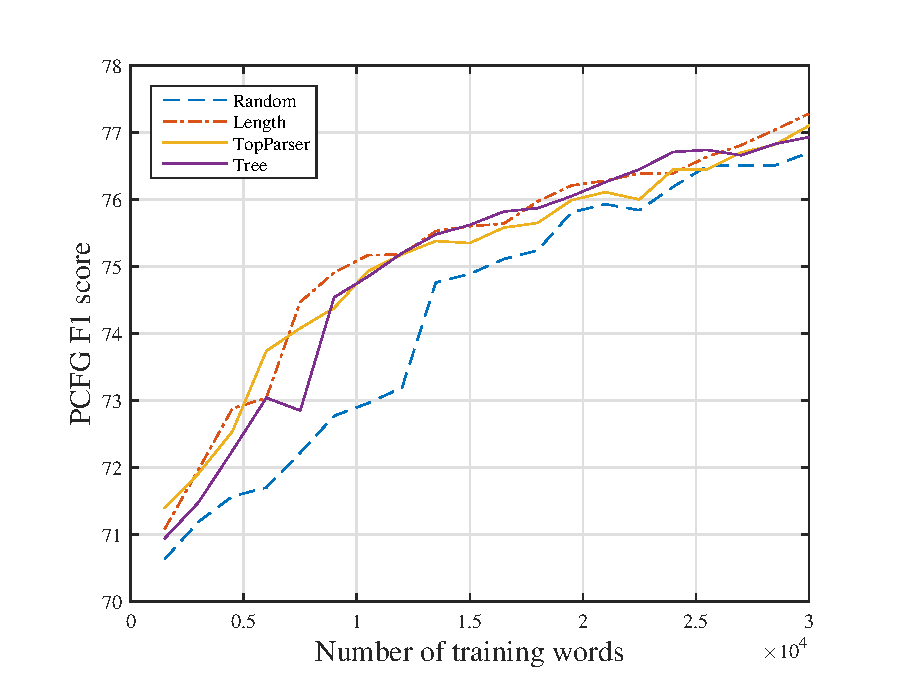
\includegraphics[scale=0.7]{basic}
\caption{Inital: first 50 sentences from section 00; Training pool: WSJ section 01 to 03; Testing: WSJ section 20; Iterations: 20; Words per each iteration: 1500.}\label{fig:basic}
\end{figure}

I got the following observations based on the results in Figure~\ref{fig:basic}: (1) 
A better selection function does lead to a good learning curve: All $T_{len}$, 
$T_{prob}$ and $T_{tree}$ outperform the baseline($T_{ran}$), especially during the early phase(word number from 1500 to 20000). This means that smart selection functions can achieve a decent 
score; (2)The tree entropy($T_{tree}$) is not as good as mentioned in~\cite{hwa}. 
Surprisingly, the naive $T_{len}$ outperforms $T_{tree}$ in words ranging from 1500
to 12000 iterations, which is different from the results of original paper. 


\subsection{Additional experiments}
I also performed additional experiments on different settings to get a better understanding of the four selection functions.

{\bf \emph{Changing the initial training set size.}} The first experiment used the same
setting as figure~\ref{fig:basic} except for using the entire 00 
section(around 100 sentences) as the initial training set. The results in 
figure~\ref{fig:init00} have similar flavour to figure~\ref{fig:basic}. The advanced
three selections still outperform the baseline($T_{ran}$), especially during early
phase(word number ranging from 1500 to 9000); The tree entropy($T_{tree}$) still doesn't show any advantage over $T_{len}$
and $T_{prob}$; If you compared it with the results in figure~\ref{fig:basic} carefully, the gap between the baseline($T_ran$) and other advanced functions reduces 
a little. 
 \begin{figure}
\centering
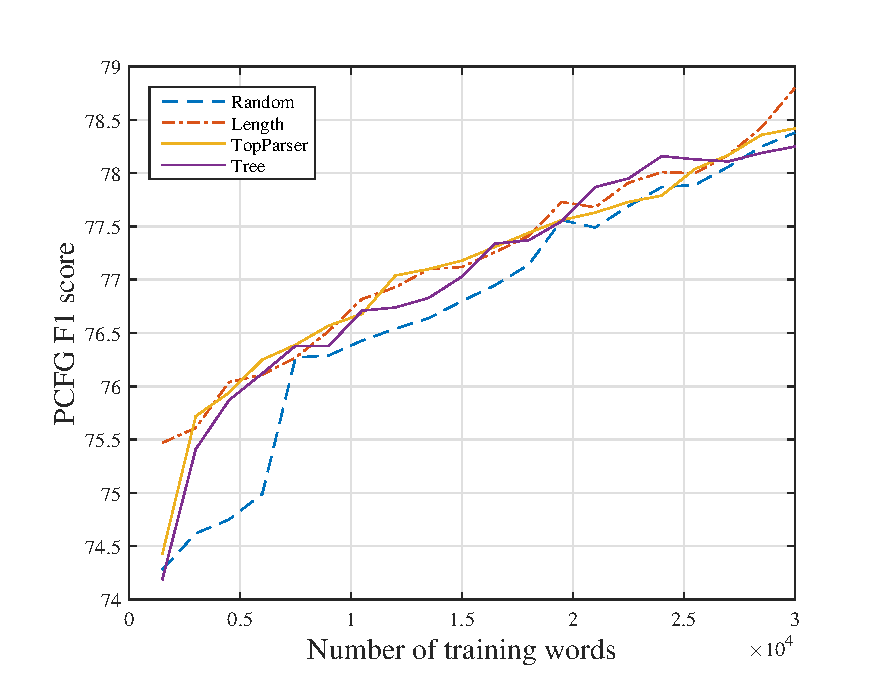
\includegraphics[scale=0.7]{init00}
\caption{Using the entire WSJ section 00 as the inital set.}\label{fig:init00}
\end{figure}

{\bf \emph{Changing the unlabeled training set.}} In the second experiment, I used 
04 to 06 sections as the new training set and other settings are identical to 
figure~\ref{fig:basic}. The results in figure~\ref{fig:train456} have a little 
difference comparing with previous two: (1)$T_{prob}$ outperforms other functions in
most iterations; (2) The baseline($T_{ran}$) is not so embarrassed any more: it 
beats $T_{len}$ and $T_{tree}$ for words ranging from 1500 to 6000; 
(3) $T_{tree}$ still doesn't show any advantage over other options. 
I still haven't figured out the reason. 
 \begin{figure}
\centering
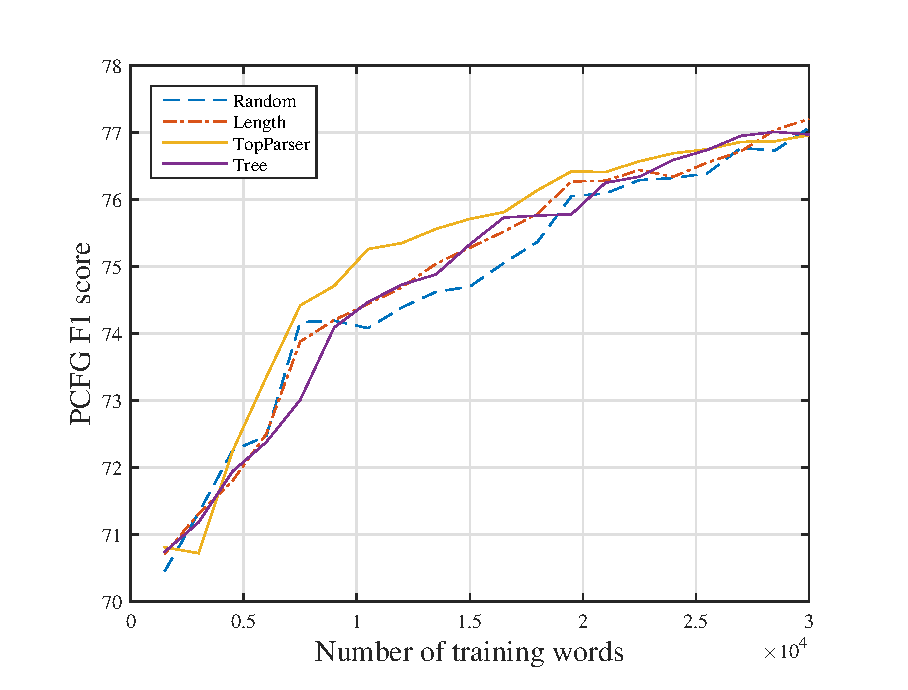
\includegraphics[scale=0.7]{train456}
\caption{Training on WSJ section 04 to 06.}\label{fig:train456}
\end{figure}

{\bf \emph{Changing the batch size for word count totals.}} In the third experiment,
I changed the batch size for word count totals from the original 1500 to 2500. 
For each iteration, the selection function has a larger window size for picking up
words so I expected that advantage of advanced selection functions over the 
baseline($T_{ran}$) should decrease. Figure~\ref{fig:bat2500} confirms this assumption. 
Surprisingly, for word number ranging from 13500 to 25000, $T_{ran}$ outperforms all
other advanced functions! Note that $T_{prob}$(TopParser) decreased strangely at 
word number 15000. I think one way to fix this is to run each selection function on the
 same setting multiple times and compute its average value. 

 \begin{figure}
\centering
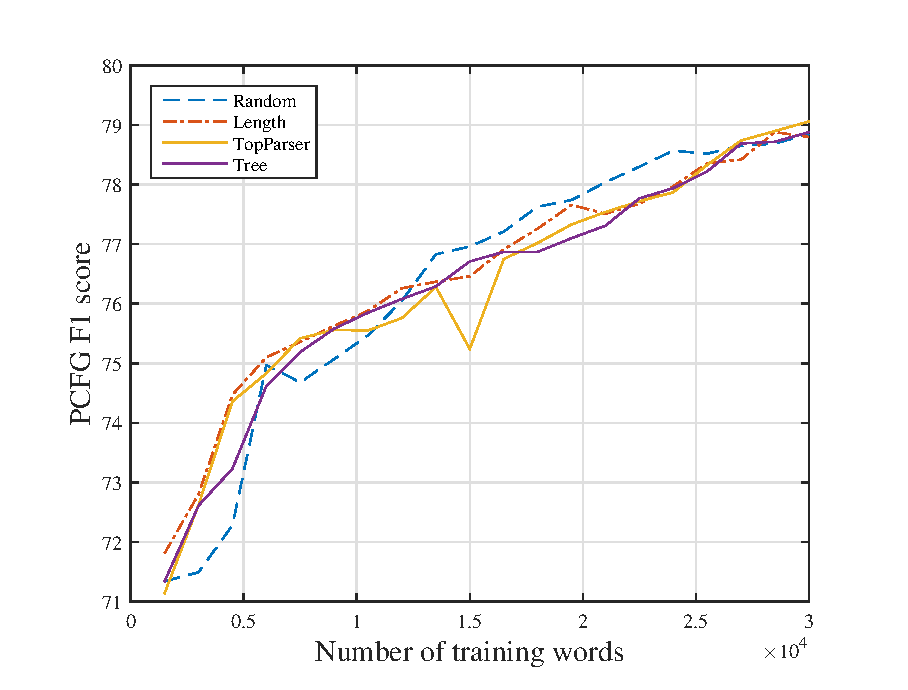
\includegraphics[scale=0.7]{bat2500}
\caption{Changing the batch size for word count totals to 2500. Other settings are identical to figure~\ref{fig:basic}}\label{fig:bat2500}
\end{figure}


{\bf \emph{Changing the Top K parses in Tree entropy.}} Even though I can't see the 
advantage of tree entropy over other selection functions in previous experiments, I 
varied different K values(5, 10, 15, 20) to study how it affects the performance.
As shown in figure~\ref{fig:topk}, it's hardly to tell which is better when the word
number is less than 20000, but after that, tree entropy with bigger K tends to yield
better results. One explanation is with a larger K value, the selection function will
take more candidate parse trees into account and make a fair decision. But the benefit of increasing value K seems not very promising.

 \begin{figure}
\centering
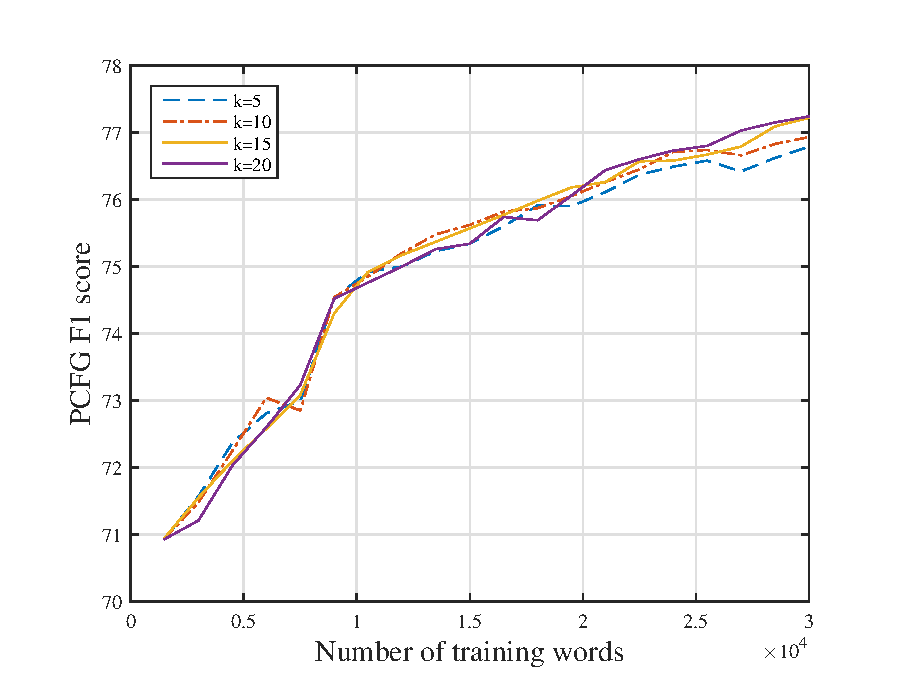
\includegraphics[scale=0.7]{topk}
\caption{Comparing the performance of different K value for the tree entropy selection.}\label{fig:topk}
\end{figure}

To conclude, even though I have explored multiple different settings to investigate
the performance of four selection functions, I still can't demonstrate the advantage 
of tree entropy over other advanced functions($T_{ran}$ and $T_{prob}$). 
Hwa's~\cite{hwa} paper shows that $T_{tree}$ strictly outperforms $T_{len}$ but in
my experiments, $T_{len}$ looks like a good choice. Combining the results in 
figure~\ref{fig:basic}, figure~\ref{fig:init00} and figure~\ref{fig:bat2500} 
together, we can observe that active learning methods achieve better learning curves
during the early phase, especially when the window size(word numbers of each iteration)
 is small. I think active learning benefits more when the parser has little knowledge
 about the training set(especially during early phase), thus achieves better learning curve. $T_{prob}$ is the best choice in figure~\ref{fig:train456} and $T_{len}$ 
 does better in figure~\ref{fig:basic}. 

\bibliographystyle{unsrt}
\bibliography{hw3}
\end{document}